%!TEX root = slides.tex

\section{Markov Chain Monte Carlo (MCMC) and Model Metrics}

\subsection{Markov Chain Monte Carlo (MCMC) and Model Metrics - Recommended References}
\begin{frame}{Markov Chain Monte Carlo (MCMC) and Model Metrics - Recommended References}
	\begin{vfilleditems}
		\item \textcite{gelman2013bayesian}
		\begin{vfilleditems}
			\item Chapter 10: Introduction to Bayesian computation
			\item Chapter 11: Basics of Markov chain simulation
			\item Chapter 12: Computationally efficient Markov chain simulation
		\end{vfilleditems}
		\item \textcite{mcelreath2020statistical} - Chapter 9: Markov Chain Monte Carlo
		\item \textcite{neal2011mcmc}
		\item \textcite{betancourtConceptualIntroductionHamiltonian2017}
		\item \textcite{gelman2020regression} - Chapter 22, Section 22.8: Computational efficiency
		\item \textcite{chibUnderstandingMetropolisHastingsAlgorithm1995}
		\item \textcite{casellaExplainingGibbsSampler1992}
	\end{vfilleditems}
\end{frame}

% \begin{frame}{Monte Carlo Methods}
% 	\begin{columns}
% 		\begin{column}{0.8\textwidth}
% 			\begin{vfilleditems}
% 				\item \href{http://mc-stan.org/}{\texttt{Stan}} is named after the mathematician Stanislaw Ulam,
% 				who was involved in the Manhattan project,
% 				and while trying to calculate the neutron diffusion process for the hydrogen bomb
% 				ended up creating a whole class of methods called \textbf{Monte Carlo} \parencite{eckhardtStanUlamJohn1987}.
% 				\item Monte Carlo methods employ randomness to solve problems in principle are deterministic in nature.
% 				They are frequently used in physics and mathematical problems,
% 				and very useful when it is difficult or impossible to use other approaches.
% 			\end{vfilleditems}
% 		\end{column}
% 		\begin{column}{0.2\textwidth}
% 			\centering
% 			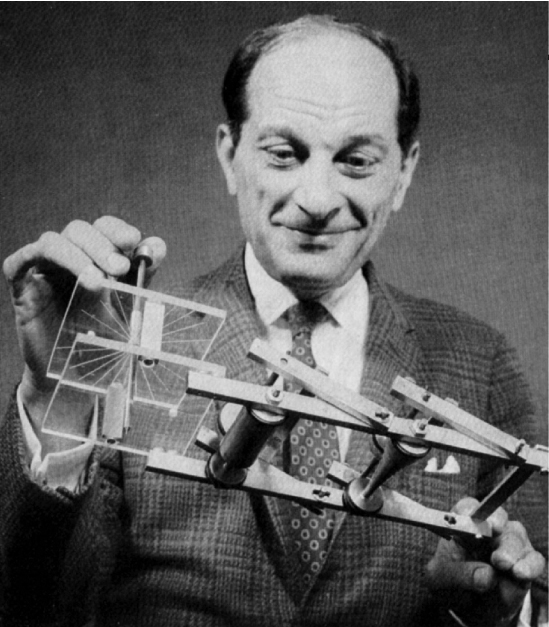
\includegraphics[width=0.9\columnwidth]{stanislaw.jpg}
% 		\end{column}
% 	\end{columns}
% \end{frame}

\begin{frame}{History Behind the Monte Carlo Methods\footnote{those who are interested, should read \textcite{eckhardtStanUlamJohn1987}.}}
	\begin{columns}
		\begin{column}{0.8\textwidth}
			\begin{vfilleditems}
				\item The idea came when Ulam was playing Solitaire while recovering from surgery.
				Ulam was trying to calculate the deterministic, i.e. analytical solution,
				of the probability of being dealt an already-won game.
				The calculations where almost impossible.
				So, he thought that he could play hundreds of games to statistically estimate,
				i.e. numerical solution, the probability of this result.
				\item Ulam described the idea to John von Neumann in 1946.
			\end{vfilleditems}
		\end{column}
		\begin{column}{0.2\textwidth}
			\centering
			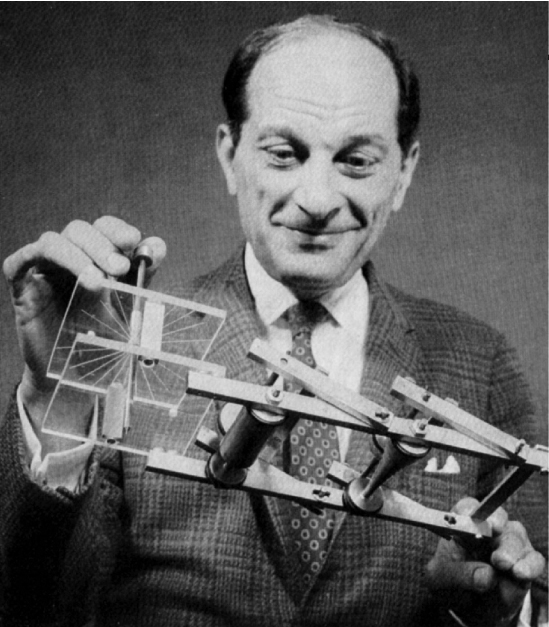
\includegraphics[width=0.9\columnwidth]{stanislaw.jpg}
		\end{column}
	\end{columns}
\end{frame}

\begin{frame}{History Behind the Monte Carlo Methods\footnote{those who are interested, should read \textcite{eckhardtStanUlamJohn1987}.}}
	\begin{columns}
		\begin{column}{0.8\textwidth}
			\begin{vfilleditems}
				\item Due to the secrecy, von Neumann and Ulam's work demanded a code name.
				Nicholas Metropolis suggested using ``Monte Carlo'',
				a homage to the ``Casino Monte Carlo'' in Monaco,
				where Ulam's uncle would ask relatives for money to play.
			\end{vfilleditems}
		\end{column}
		\begin{column}{0.2\textwidth}
			\centering
			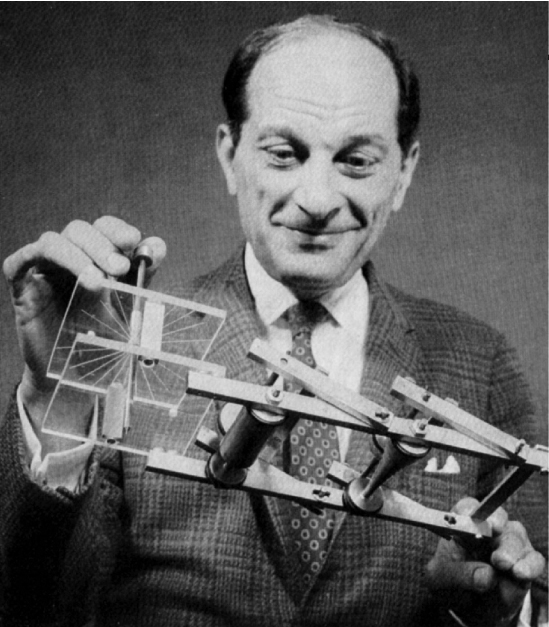
\includegraphics[width=0.9\columnwidth]{stanislaw.jpg}
		\end{column}
	\end{columns}
\end{frame}

\subsection{Why Do We Need MCMC?}
\begin{frame}{Why Do We Need MCMC?}
	The main computation barrier for Bayesian statistics is the denominator in Bayes' theorem,
	$P(\text{data})$:
	$$
		P(\theta \mid \text{data})=\frac{P(\theta) \cdot P(\text{data} \mid \theta)}{P(\text{data})}
	$$
	In finite, discrete cases, we can turn the denominator into a sum over a finite number of combinations of parameters.
	Let $N$ resemble the number of combinations of parameter values and let $\theta_i$ resemble a particular vector of such combination. Using the \textbf{chain rule} of probability:
	$$
		P(\text{data}, \theta_1) = P(\theta_1) \cdot P(\text{data} \mid \theta_1)
	$$
\end{frame}

\begin{frame}{Why Do We Need MCMC?}
	We can then \textbf{marginalize} the random variable $\theta$ using:
	$$
		P(\text{data}) = \sum_{i}^N P(\text{data}, \theta_i) = \sum_{i}^N P(\theta_i) \cdot P(\text{data} \mid \theta_i)
	$$
	\vfill
	In the non-finite cases (domains are not compact, e.g. they go to $\infty$ or $-\infty$), this turns into an infinite series which can still be tractable (computationally feasible) sometimes.
	\vfill
	In the continuous case, this turns into an integral over all values of $\theta$.
	$$
		P(\text{data})=\int_{\theta} P(\text{data} \mid \theta) \times P(\theta)d \theta
	$$
\end{frame}

\begin{frame}{Why Do We Need MCMC?}
	$$
		P(\text{data})=\int_{\theta} P(\text{data} \mid \theta) \times P(\theta)d \theta
	$$
	In many cases, e.g. if $\theta$ is high dimensional, this integral (or sum in the discrete case) is intractable.
	That is, it is not feasible to deterministically evaluate or even approximate it to a known residual error.
	Therefore, we must find other ways to compute and use the posterior
	$P(\theta \mid \text{data})$ without using the denominator
	$P(\text{data})$.
	\vfill
	\Large \textbf{This is where Monte Carlo methods come into play!}
\end{frame}

\begin{frame}{Why Do We Need the Denominator $P(\text{data})$?}
	To normalize the posterior with the intent of making it a \textbf{valid probability}.
	This means that the probability for all possible parameters' values must be $1$:
	\begin{vfilleditems}
		\item in the \textbf{discrete} case:
		$$
			\sum_{\theta} P(\theta \mid \text{data}) = 1
		$$
		\item in the \textbf{continuous} case:
		$$
			\int_{\theta} P(\theta \mid \text{data})d \theta = 1
		$$
	\end{vfilleditems}
	$P(\text{data})$ also gives us a measure of the total likelihood of a model class. This is useful when considering and comparing multiple models.
\end{frame}

\begin{frame}{Why Do We Need the Denominator $P(\text{data})$?}
	\begin{vfilleditems}
		\item After evaluating $P(\text{data})$, we still need to evaluate more integrals over $\theta$.
		\item A lot of useful questions can be formulated as such integrals.
		\item The probability $P(\theta > 0 | \text{data})$ according to the posterior is:
		$$
			\int_{\theta} 1_{\theta > 0} \, P(\theta \mid \text{data}) d\theta
		$$
		where $1_{\theta > 0}$ is 1 if $\theta > 0$ and 0 otherwise.
		\item The expected prediction $y(\theta)$ which is a function of the parameters $\theta$ given the posterior distribution is:
		$$
			\int_{\theta} y(\theta) \, P(\theta \mid \text{data}) d\theta
		$$
		\item All those integrals are typically intractable for high dimensional $\theta$.
	\end{vfilleditems}
\end{frame}

\begin{frame}{Sampling from the posterior}
	\begin{vfilleditems}
		\item What if we have a way to sample from the posterior distribution $P(\theta \mid \text{data})$ without evaluating $P(\text{data})$ or any of the above integrals?
		\item Can we answer our useful questions?
		\item Let the number of samples from the posterior be $N$ and let $\theta_i$ be the $i^{th}$ sample from the posterior.
		$$
			\int_{\theta} 1_{\theta > 0} \, P(\theta \mid \text{data}) d\theta \approx \frac{1}{N} \sum_i^N 1_{\theta_i > 0}
		$$
		$$
			\int_{\theta} y(\theta) \, P(\theta \mid \text{data}) d\theta \approx \frac{1}{N} \sum_i^N y(\theta_i)
		$$
		\item These are all tractable sums!
	\end{vfilleditems}
\end{frame}

\begin{frame}{What If We Remove the Denominator $P(\text{data})$?}
	By removing the denominator $P(\text{data})$,
	we conclude that the posterior

	$P(\theta \mid \text{data})$ is \textbf{proportional} to the
	product of the prior and the likelihood
	$P(\theta) \cdot P(\text{data} \mid \theta)$:
	$$
		P(\theta \mid \text{data}) \propto P(\theta, \text{data}) = P(\theta) \cdot P(\text{data} \mid \theta)
	$$
\end{frame}

\subsubsection{Markov Chains}
\begin{frame}{Markov Chain Monte Carlo (MCMC)}
	Here is where \textbf{Markov Chain Monte Carlo} comes in:
	\vfill
	MCMC is an ample class of computational tools to approximate integrals
	and generate samples from a posterior probability
	\parencite{brooksHandbookMarkovChain2011} using nothing but the un-normalized probability $P(\theta, \text{data})$.
	\vfill
	MCMC is used when it is not possible to sample $\boldsymbol{\theta}$
	directly from the posterior probability
	$P(\boldsymbol{\theta} \mid \text{data})$.
	Instead, we collect samples in an iterative manner,
	where every step of the process we expect that the distribution which we are sampling from
	$P^*(\boldsymbol{\theta}^{(*)} \mid \text{data})$
	becomes more similar in every iteration to the posterior
	$P(\boldsymbol{\theta} \mid \text{data})$.
	\vfill
	All of this is to \textbf{eliminate the evaluation}
	(often impossible) of the intractable integrals.
\end{frame}

\begin{frame}{Markov Chains}
	\begin{columns}
		\begin{column}{0.8\textwidth}
			\begin{vfilleditems}
				\item We proceed by defining an \textbf{ergodic Markov chain}\footnotemark.
				in which the set of possible states is the sample size and
				the stationary distribution is the distribution to be \textit{approximated}
				(or \textit{sampled}).
				\item Let $X_0, X_1, \dots, X_n$ be a simulation of the chain.
				The Markov chain \textbf{converges to the stationary distribution from any initial state}
				$X_0$ after a \textbf{sufficient large number of iterations} $r$.
				The distribution of the state $X_r$ will be similar to the stationary distribution,
				hence we can use it as a sample.
			\end{vfilleditems}
		\end{column}
		\begin{column}{0.2\textwidth}
			\centering
			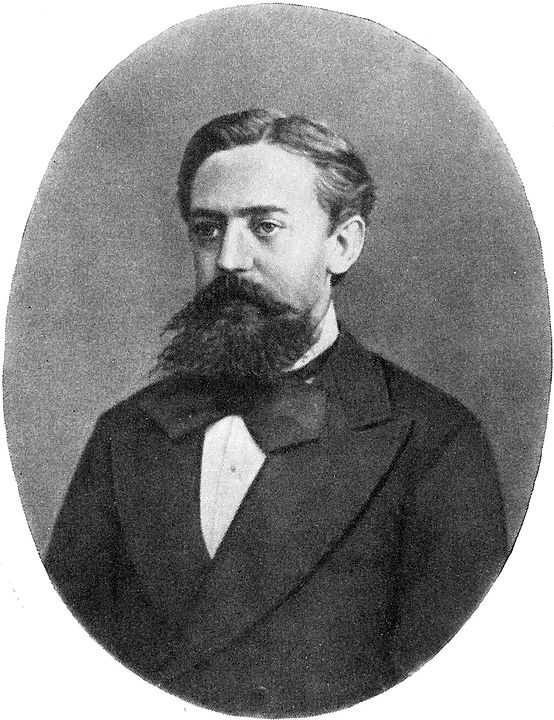
\includegraphics[width=0.9\columnwidth]{andrei_markov.jpg}
		\end{column}
	\end{columns}
	\footnotetext{meaning that there is an \textbf{unique stationary distribution}}
\end{frame}

\begin{frame}{Markov Chains}
	\begin{columns}
		\begin{column}{0.8\textwidth}
			\begin{vfilleditems}
				\item Markov chains have a property that the probability distribution of the next state
				\textbf{depends only on the current state and not in the sequence of events that preceded}:
				$$
					P(X_{n+1}=x \mid X_{0},X_{1},X_{2},\ldots ,X_{n}) = P(X_{n+1}=x \mid X_{n})
				$$
				This property is called \textbf{Markovian}
				\item Similarly, using this argument with $X_r$ as the initial state,
				we can use $X_{2r}$ as a sample, and so on.
				We can use the sequence of states $X_r, X_{2r}, X_{3r}, \dots$
				as almost \textbf{independent samples} of Markov chain stationary distribution.
			\end{vfilleditems}
		\end{column}
		\begin{column}{0.2\textwidth}
			\centering
			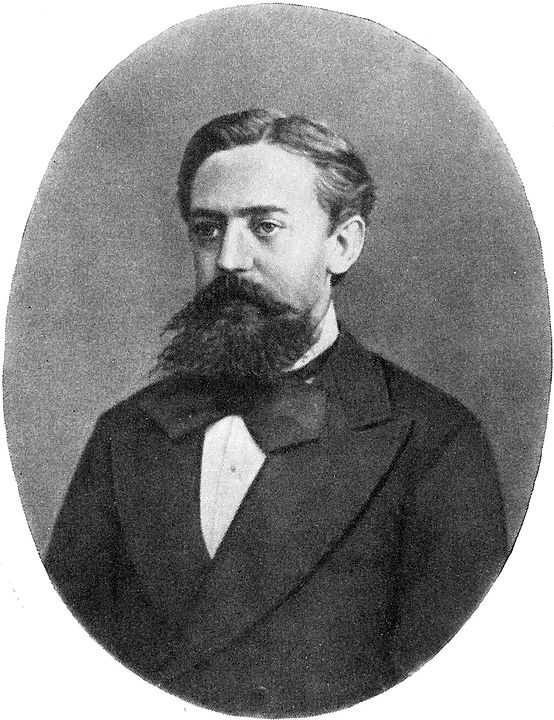
\includegraphics[width=0.9\columnwidth]{andrei_markov.jpg}
		\end{column}
	\end{columns}
\end{frame}

% Idea taken from http://steventhornton.ca/blog/markov-chains-in-latex.html
\begin{frame}{Example of a Markov Chain}
	\centering
	\begin{tikzpicture}
		% Add the states
		\node[state,
			text=yellow,
			minimum size=2cm,
			thick
		]
		(s) {Sun};
		\node[state,
			right=3cm of s,
			text=blue!30!white,
			minimum size=2cm,
			thick
		]
		(r) {Rain};

		% Connect the states with arrows
		\draw[every loop,
			auto=right,
			line width=1mm,
			>=latex]
		(s) edge[bend right, auto=left]  node {0.6} (r)
		(r) edge[bend right, auto=right] node {0.7} (s)
		(s) edge[loop above]             node {0.4} (s)
		(r) edge[loop above]             node {0.3} (r);
	\end{tikzpicture}
\end{frame}

\begin{frame}{Markov Chains}
	The efficacy of this approach depends on:
	\begin{vfilleditems}
		\item \textbf{how big $r$ must be} to guarantee an \textbf{adequate sample}.
		\item \textbf{computational power} required for every Markov chain iteration.
	\end{vfilleditems}

	\vfill
	\footnotesize
	Besides, it is custom to discard the first iterations of the algorithm because
	they are usually non-representative of the underlying stationary distribution to be approximate.
	In the initial iterations of MCMC algorithms,
	often the Markov chain is in a ``warm-up''\footnote{some references call this ``burnin''.} process,
	and its state is very far away from an ideal one to begin a trustworthy sampling.
	\vfill
	Generally, it is recommended to \textbf{discard the first half iterations} \parencite{gelmanBasicsMarkovChain2013}.
\end{frame}

\subsection{MCMC Algorithms}
\begin{frame}{MCMC Algorithms}\
	MCMC algorithms\footnote{see the \href{https://en.wikipedia.org/wiki/Markov_chain_Monte_Carlo}{Wikipedia page for a full list}.} use a Markov chain that's guaranteed to converge to the target posterior distribution $P(\theta \mid \text{data}$ using nothing but the un-normalized probability $P(\theta, \text{data})$.
	\vfill
	We have \textbf{TONS} of MCMC algorithms.
	Here we are going to cover two classes of MCMC algorithms:
	\begin{vfilleditems}
		\item Metropolis-Hastings \parencite{metropolisEquationStateCalculations1953, hastingsMonteCarloSampling1970}.
		\item Hamiltonian Monte Carlo\footnote{sometimes called Hybrid Monte Carlo, specially in the physics literature.} \parencite{neal2011mcmc, betancourtConceptualIntroductionHamiltonian2017}.
	\end{vfilleditems}
\end{frame}


\subsubsection{Metropolis}
\begin{frame}{Metropolis Algorithm}
	\begin{columns}
		\begin{column}{0.8\textwidth}
			The first broadly used MCMC algorithm to generate samples from a Markov chain
			was originated in the physics literature in the 1950s and is called Metropolis
			\parencite{metropolisEquationStateCalculations1953},
			in honor of the first author
			\href{https://en.wikipedia.org/wiki/Nicholas_Metropolis}{Nicholas Metropolis}.
			\vfill
			In sum, the Metropolis algorithm is an adaptation of a random walk coupled
			with an acceptance/rejection rule to converge to the target distribution.
			\vfill
			Metropolis algorithm uses a \textbf{proposal distribution}
			$J_t(\boldsymbol{\theta}^{(*)})$
			to define the next values of the distribution
			$P^*(\boldsymbol{\theta}^{(*)} \mid \text{data})$.
			This distribution must be symmetric:
			$$
				J_t (\boldsymbol{\theta}^{(*)} \mid \boldsymbol{\theta}^{(t-1)}) = J_t(\boldsymbol{\theta}^{(t-1)} \mid \boldsymbol{\theta}^{(*)})
			$$
		\end{column}
		\begin{column}{0.2\textwidth}
			\centering
			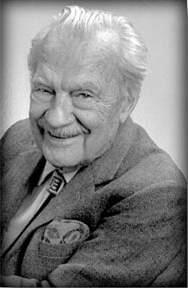
\includegraphics[width=0.9\columnwidth]{nicholas_metropolis.png}
		\end{column}
	\end{columns}
\end{frame}

\begin{frame}{Metropolis Algorithm}
	Metropolis is a random walk through the parameter sample space,
	where the probability of the Markov chain changing its state is defined as:
	$$
		P_{\text{change}} = \min\left({\frac{P (\boldsymbol{\theta}_{\text{proposed}})}{P (\boldsymbol{\theta}_{\text{current}})}},1\right).
	$$
	This means that the Markov chain will only change to a new state based in one of two conditions:
	\begin{vfilleditems}
		\small
		\item when the probability of the random walk proposed parameters
		$P(\boldsymbol{\theta}_{\text{proposed}})$ is \textbf{\textcolor{blue}{higher}}
		than the probability of the current state parameters
		$P(\boldsymbol{\theta}_{\text{current}})$,
		we change with 100\% probability.
		\item when the probability of the random walk proposed parameters
		$P(\boldsymbol{\theta}_{\text{proposed}})$ is \textbf{\textcolor{red}{lower}}
		than the probability of the current state parameters
		$P(\boldsymbol{\theta}_{\text{current}})$,
		we change with probability equal to the proportion of this probability difference.
	\end{vfilleditems}
\end{frame}

\begin{frame}{Metropolis Algorithm}
	\SetAlCapFnt{\normalsize}
	\SetAlCapNameFnt{\normalsize}
	\begin{algorithm}[H]
		\DontPrintSemicolon
		\SetAlgoNoEnd
		\SetAlgoLined
		Define an initial set $\boldsymbol{\theta}^{(0)} \in \mathbb{R}^p$ that $P\left(\boldsymbol{\theta}^{(0)} \mid \mathbf{y} \right) > 0$\;
		\For{$t = 1, 2, \dots$}{
			Sample a proposal of $\boldsymbol{\theta}^{(*)}$ from a proposal distribution in time $t$, $J_t \left(\boldsymbol{\theta}^{(*)} \mid \boldsymbol{\theta}^{(t-1)} \right)$\;
			As an acceptance/rejection rule, compute the proportion of the probabilities:
			$r = \frac{P\left(\boldsymbol{\theta}^{(*)}  \mid \mathbf{y} \right)}{P\left(\boldsymbol{\theta}^{(t-1)} \mid \mathbf{y} \right)}$\;
			Assign:
			$
				\boldsymbol{\theta}^{(t)} =
				\begin{cases}
					\boldsymbol{\theta}^{(*)}   & \text{with probability $\min(r,1)$} \\
					\boldsymbol{\theta}^{(t-1)} & \text{otherwise}
				\end{cases}
			$\;
		}
		\caption{Metropolis}
	\end{algorithm}
\end{frame}

\begin{frame}{Visual Intuition -- Metropolis}
	\centering
	\begin{tikzpicture}
		\begin{axis}[every axis plot, line width=2pt,
				ylabel=PDF,
				domain=-4:4,samples=200,
				ymax = 0.6, ytick={0, 0.2, 0.4},
				axis x line*=bottom, % no box around the plot, only x and y axis
				axis y line*=left, % the * suppresses the arrow tips
				enlargelimits=true,
			] % extend the axes a bit

			\addplot [blue] {gaussian(0, 1)};
			\node[inner sep=0pt] (hikerlower) at (-2,0.13){\Strichmaxerl[2pt]};
			\node[inner sep=0pt] (hikerupper) at (0,0.5){\Strichmaxerl[2pt]};
			\node[inner sep=0pt] (hikerlower2) at (2,0.13){\Strichmaxerl[2pt]};
			\draw[->, red, line width=2pt] (hikerlower) to [out=90,in=135] node[above left] {\large$P=1$} (hikerupper);
			\draw[->, yellow, line width=2pt] (hikerupper) to [out=45,in=135] node[right] {\large$P\approx\frac{0.1}{0.4}\approx\frac{1}{4}$} (hikerlower2);
		\end{axis}
	\end{tikzpicture}
\end{frame}

\subsubsection{Metropolis-Hastings (MH)}
\begin{frame}{Metropolis-Hastings Algorithm}
	\begin{columns}
		\begin{column}{0.8\textwidth}
			In the 1970s emerged a generalization of the Metropolis algorithm,
			which \textbf{does not need that the proposal distributions be symmetric}:
			$$
				J_t (\boldsymbol{\theta}^{(*)} \mid \boldsymbol{\theta}^{(t-1)}) \neq J_t(\boldsymbol{\theta}^{(t-1)} \mid \boldsymbol{\theta}^{(*)})
			$$
			The generalization was proposed by \href{https://en.wikipedia.org/wiki/W._K._Hastings}{Wilfred Keith Hastings}
			\parencite{hastingsMonteCarloSampling1970} and is called \textbf{Metropolis-Hastings algorithm}.
		\end{column}
		\begin{column}{0.2\textwidth}
			\centering
			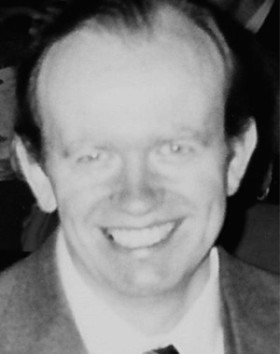
\includegraphics[width=0.9\columnwidth]{hastings.jpg}
		\end{column}
	\end{columns}
\end{frame}

\begin{frame}{Metropolis-Hastings Algorithm}
	\SetAlCapFnt{\normalsize}
	\SetAlCapNameFnt{\normalsize}
	\small
	\begin{algorithm}[H]
		\DontPrintSemicolon
		\SetAlgoNoEnd
		\SetAlgoLined
		Define an initial set $\boldsymbol{\theta}^{(0)} \in \mathbb{R}^p$ that $P\left(\boldsymbol{\theta}^{(0)} \mid \mathbf{y} \right) > 0$\;
		\For{$t = 1, 2, \dots$}{
			Sample a proposal $\boldsymbol{\theta}^{(*)}$ from a proposal distribution in time $t$, $J_t \left(\boldsymbol{\theta}^{(*)} \mid \boldsymbol{\theta}^{(t-1)} \right)$\;
			As an acceptance/rejection rule, compute the proportion of the probabilities:
			$r = \frac{\frac{P \left(\boldsymbol{\theta}^{(*)} \mid \mathbf{y} \right)}{J_t \left(\boldsymbol{\theta}^{(*)} \mid \boldsymbol{\theta}^{(t-1)} \right)}}{\frac{P \left(\boldsymbol{\theta}^{(t-1)} \mid \mathbf{y} \right)}{J_t \left(\boldsymbol{\theta}^{(t-1)} \mid \boldsymbol{\theta}^{(*)} \right)}}$\;
			Assign:
			$
				\boldsymbol{\theta}^{(t)} =
				\begin{cases}
					\boldsymbol{\theta}^{(*)}   & \text{with probability $\min(r,1)$} \\
					\boldsymbol{\theta}^{(t-1)} & \text{otherwise}
				\end{cases}
			$\;
		}
		\caption{Metropolis-Hastings}
	\end{algorithm}
\end{frame}

% \begin{frame}{Metropolis-Hastings Animation\footnote{see Metropolis-Hastings in action at \href{https://chi-feng.github.io/mcmc-demo/app.html?algorithm=RandomWalkMH&target=banana}{\texttt{chi-feng/mcmc-demo}}.}}
% 	\centering
% 	\movie[loop, width=9cm, height=6cm]{Metropolis Animation}{animations/rwmh.m4v}
% \end{frame}

\begin{frame}{Metropolis-Hastings Animation}
	See Metropolis-Hastings in action at \href{https://chi-feng.github.io/mcmc-demo/app.html?algorithm=RandomWalkMH&target=banana}{\texttt{chi-feng/mcmc-demo}}.
\end{frame}

\subsubsection{Limitations of the Metropolis Algorithms}
\begin{frame}{Limitations of the Metropolis Algorithms}
	The limitations of the Metropolis-Hastings algorithms are mainly \textbf{computational}:
	\begin{vfilleditems}
		\item with the proposals randomly generated,
		it can take a large number of iterations for the
		Markov chain to enter higher posterior densities spaces.
		\item even highly-efficient MH algorithms sometimes accept \textbf{less than}
		25\% of the proposals in the Gaussian case \parencite{robertsWeakConvergenceOptimal1997, beskosOptimalTuningHybrid2013}, often much less in complicated models.
		\item in lower-dimensional contexts, higher computational power can compensate the low efficiency up to a point.
		But in higher-dimensional (and higher-complexity) modeling situations,
		higher computational power alone are rarely sufficient to overcome the low efficiency.
	\end{vfilleditems}
\end{frame}

% \begin{frame}{MCMC Algorithms -- Metropolis-Hastings}
% 	These are the first MCMC algorithms.
% 	They use an \textbf{acceptance/rejection rule for the proposals}.
% 	They are characterized by proposals originated from a random walk in the parameter space.

% 	The \textbf{Gibbs algorithm} can be seen as a \textbf{special case} of MH
% 	because all proposals are automatically accepted \parencite{gelmanIterativeNonIterativeSimulation1992}
% 	\vfill
% 	Asymptotically, they have an acceptance rate of 23.4\%,
% 	and the computational cost of every iteration is $\mathcal{O}(d)$,
% 	where $d$ is the number of dimension in the parameter space \parencite{beskosOptimalTuningHybrid2013}.
% \end{frame}

\begin{frame}{Hamiltonian Monte Carlo (HMC)}
	The current most efficient MCMC algorithms for continuous parameters.
	They try to \textbf{avoid the entirely random walk behavior by introducing an auxiliary vector of random momenta
		using Hamiltonian dynamics}.
	The proposals (albeit still random) are then ``guided'' to higher density regions of the sample space.
	This makes \textbf{HMC more efficient by multiple orders of magnitude when compared to MH}.
	% \vfill
	% Asymptotically, they have an acceptance rate of 65.1\%,
	% and the computational cost of every iteration is $\mathcal{O}(d^{\frac{1}{4}})$,
	% where $d$ is the number of dimension in the parameter space \parencite{beskosOptimalTuningHybrid2013}.
\end{frame}

% \subsubsection{Gibbs}
% \begin{frame}{Gibbs Algorithm}
% 	\begin{columns}
% 		\begin{column}{0.8\textwidth}
% 			To circumvent Metropolis' low acceptance rate, the Gibbs algorithm was conceived.
% 			Gibbs \textbf{do not have an acceptance/rejection rule} for the Markov chain state change:
% 			\textbf{all proposals are accepted!}
% 			\vfill
% 			Gibbs algorithm was originally conceived by the physicist Josiah Willard Gibbs
% 			while referencing an analogy between a sampling algorithm and
% 			statistical physics (a physics field that originates from statistical mechanics).
% 			The algorithm was described by the Geman brothers in 1984
% 			\parencite{gemanStochasticRelaxationGibbs1984},
% 			about 8 decades after Gibbs death.
% 		\end{column}
% 		\begin{column}{0.2\textwidth}
% 			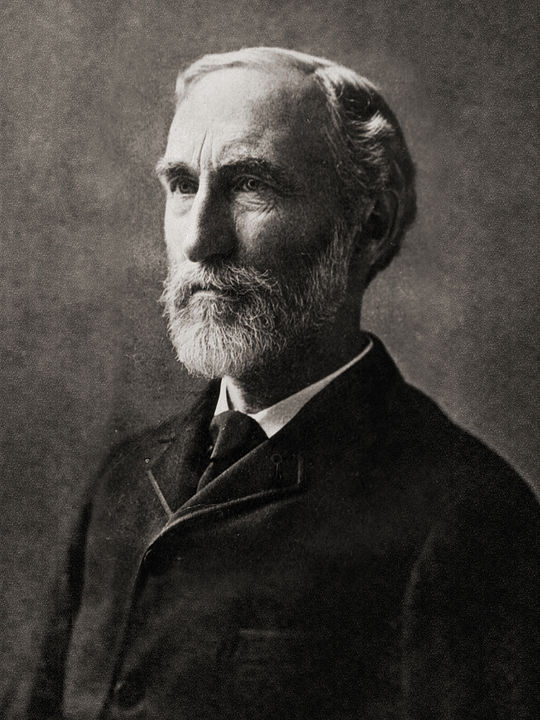
\includegraphics[width=0.9\columnwidth]{josiah_gibbs.jpg}
% 		\end{column}
% 	\end{columns}
% \end{frame}

% \begin{frame}{Gibbs Algorithm}
% 	The Gibbs algorithm is very useful in multidimensional sample spaces.
% 	It is also known as \textbf{alternating conditional sampling},
% 	because we always sample a parameter \textbf{conditioned} on the probability of the other model's parameters.
% 	\vfill
% 	The Gibbs algorithm can be seen as a \textbf{special case} of the Metropolis-Hastings algorithm,
% 	because all proposals are accepted
% 	\parencite{gelmanIterativeNonIterativeSimulation1992}.
% 	\vfill
% 	The essence of the Gibbs algorithm is the sampling of parameters conditioned in other parameters:
% 	$$P(\theta_1 \mid \theta_2, \dots \theta_p)$$
% \end{frame}

% \begin{frame}[fragile]{Gibbs Algorithm}
% 	\SetAlCapFnt{\normalsize}
% 	\SetAlCapNameFnt{\normalsize}
% 	\begin{algorithm}[H]
% 		\DontPrintSemicolon
% 		\SetAlgoNoEnd
% 		\SetAlgoLined
% 		Define an initial set $\boldsymbol{\theta}^{(0)} \in \mathbb{R}^p$ that $P\left(\boldsymbol{\theta}^{(0)} \mid \mathbf{y} \right) > 0$\;
% 		\For{$t = 1, 2, \dots$}{
% 			Assign:
% 			$ \boldsymbol{\theta}^{(t)} =
% 				\begin{cases}
% 					\theta^{(t)}_1 & \sim P \left(\theta_1 \mid \theta^{(0)}_2, \dots, \theta^{(0)}_p \right)         \\
% 					\theta^{(t)}_2 & \sim P \left(\theta_2 \mid \theta^{(t-1)}_1, \dots, \theta^{(0)}_p \right)       \\
% 					               & \vdots                                                                           \\
% 					\theta^{(t)}_p & \sim P \left(\theta_p \mid \theta^{(t-1)}_1, \dots, \theta^{(t-1)}_{p-1} \right)
% 				\end{cases}
% 			$\;
% 		}
% 		\caption{Gibbs}
% 	\end{algorithm}
% \end{frame}

% \begin{frame}{Gibbs Animation\footnote{see Gibbs in action at \href{https://chi-feng.github.io/mcmc-demo/app.html?algorithm=GibbsSampling&target=banana}{\texttt{chi-feng/mcmc-demo}}.}}
% 	\centering
% 	\movie[loop, width=9cm, height=6cm]{Gibbs Animation}{animations/gibbs.m4v}
% \end{frame}

% \subsubsection{Limitations of the Gibbs Algorithm}
% \begin{frame}{Limitations of the Gibbs Algorithm}
% 	The main limitation of Gibbs algorithm is with relation to
% 	\textbf{alternating conditional sampling}:
% 	\begin{vfilleditems}
% 		\item In Metropolis, the parameters' random proposals are sampled
% 		\textbf{unconditionally}, \textbf{jointly}, and \textbf{simultaneous}.
% 		The Markov chain state changes are executed in a
% 		\textbf{multidimensional} manner.
% 		This makes \textbf{multidimensional diagonal movements}.
% 		\item In the case of the Gibbs algorithm,
% 		this movement only happens one parameter at a time,
% 		because we sample parameters in a
% 		\textbf{conditional} and \textbf{sequential} manner with respect
% 		to other parameters.
% 		This makes \textbf{unidimensional horizontal/vertical movements},
% 		and never multidimensional diagonal movements.
% 	\end{vfilleditems}
% \end{frame}

\subsubsection{Hamiltonian Monte Carlo (HMC)}
\begin{frame}{Hamiltonian Monte Carlo (HMC)}
	\begin{columns}
		\begin{column}{0.8\textwidth}
			Metropolis' low acceptance rate in multidimensional problems
			(where the posterior geometry is highly complex)
			made a new class of MCMC algorithms emerge.
			These are called Hamiltonian Monte Carlo (HMC),
			because they incorporate Hamiltonian dynamics
			(in honor of Irish physicist
			\href{https://en.wikipedia.org/wiki/William_Rowan_Hamilton}{William Rowan Hamilton}).
		\end{column}
		\begin{column}{0.2\textwidth}
			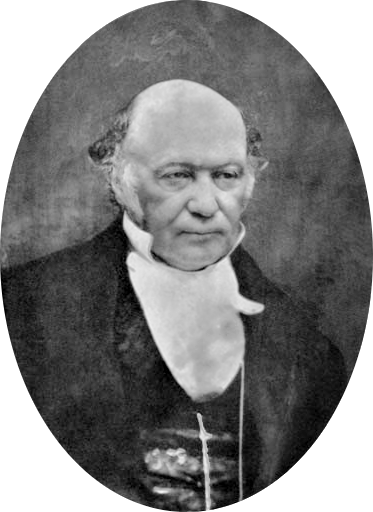
\includegraphics[width=0.9\columnwidth]{hamilton.png}
		\end{column}
	\end{columns}
\end{frame}

\begin{frame}{HMC Algorithm}
	HMC algorithm is an adaptation of the MH algorithm,
	and employs a guidance scheme to the generation of new proposals.
	It boosts the acceptance rate, and, consequently, has a better efficiency.
	\vfill
	More specifically, HMC uses the gradient of the posterior's log density
	to guide the Markov chain to higher density regions of the sample space,
	where most of the samples are sampled:
	$$
		\frac{d \log P(\boldsymbol{\theta} \mid \mathbf{y})}{d \theta}
	$$
	As a result, a Markov chain that uses a well-adjusted HMC algorithm will accept
	proposals with a much higher rate than if using the MH algorithm
	\parencite{robertsWeakConvergenceOptimal1997, beskosOptimalTuningHybrid2013}.
\end{frame}

\begin{frame}{History of HMC Algorithm}
	HMC was originally described in the physics literature\footnote{where is called ``Hybrid'' Monte Carlo (HMC)}
	\parencite{duaneHybridMonteCarlo1987}.
	\vfill
	Soon after, HMC was applied to statistical problems by
	\textcite{nealImprovedAcceptanceProcedure1994} who named it as Hamiltonian Monte Carlo (HMC).
	\vfill
	For a much more detailed and in-depth discussion (not our focus here) of HMC,
	I recommend
	\textcite{neal2011mcmc} and \textcite{betancourtConceptualIntroductionHamiltonian2017}.
\end{frame}

\begin{frame}{What Changes With HMC?}
	HMC uses Hamiltonian dynamics applied to particles efficiently exploring
	a posterior probability geometry,
	while also being robust to complex posterior's geometries.
	\vfill
	Besides that, HMC is much more efficient than Metropolis
	% and does \textit{not} suffer Gibbs' parameters correlation issues
\end{frame}

\begin{frame}{Intuition Behind the HMC Algorithm}
	\small
	For every parameter $\theta_j$, HMC adds a momentum variable $\phi_j$.
	The posterior density $P(\boldsymbol{\theta} \mid y)$ is incremented by an
	independent momenta distribution $P(\boldsymbol{\phi})$,
	hence defining the following joint probability:
	$$
		P(\boldsymbol{\theta}, \boldsymbol{\phi} \mid y) = P(\boldsymbol{\phi}) \cdot P(\boldsymbol{\theta} \mid y)
	$$
	\small
	HMC uses a proposal distribution that changes depending on the Markov chain current state.
	HMC finds the direction where the posterior density increases,
	the \textbf{gradient},
	and alters the proposal distribution towards the gradient direction.
	\vfill
	The probability of the Markov chain to change its state in HMC is defined as:
	$$
		P_{\text{change}} = \min\left({\frac{P(\boldsymbol{\theta}_{\text{proposed}}) \cdot P(\boldsymbol{\phi}_{\text{proposed}})}{P(\boldsymbol{\theta}_{\text{current}})\cdot P(\boldsymbol{\phi}_{\text{current}})}}, 1\right)
	$$
\end{frame}

\begin{frame}{Momenta Distribution -- $P(\boldsymbol{\phi})$}
	Generally we give $\boldsymbol{\phi}$ a multivariate normal distribution
	with mean $0$ and covariance$\mathbf{M}$,
	a ``mass matrix''.
	\vfill
	To keep things computationally simple,
	we used a \textbf{diagonal} mass matrix $\mathbf{M}$.
	This makes that the diagonal elements (components) $\boldsymbol{\phi}$ are independent,
	each one having a normal distribution:
	$$\phi_j \sim \text{Normal}(0, M_{jj})$$
\end{frame}

\begin{frame}[fragile]{HMC Algorithm}
	\SetAlCapFnt{\normalsize}
	\SetAlCapNameFnt{\normalsize}
	\begin{algorithm}[H]
		\DontPrintSemicolon
		\SetAlgoNoEnd
		\SetAlgoLined
		\footnotesize
		Define an initial set $\boldsymbol{\theta}^{(0)} \in \mathbb{R}^p$ that $P\left(\boldsymbol{\theta}^{(0)} \mid \mathbf{y} \right) > 0$\;
		Sample $\boldsymbol{\phi}$ from a $\text{Multivariate Normal}(\mathbf{0},\mathbf{M})$\;
		Simultaneously sample $\boldsymbol{\theta}^{(*)}$ and $\boldsymbol{\phi}$ with $L$ steps and step-size $\epsilon$.\;
		Define the current value of $\boldsymbol{\theta}$ as the proposed value $\boldsymbol{\theta}^{(*)}$:
		$\boldsymbol{\theta}^{(*)} \leftarrow \boldsymbol{\theta}$\;
		\For{$1, 2, \dots, L$}{
			Use the $\log$ of the posterior's gradient $\boldsymbol{\theta}^{(*)}$ to produce a half-step of $\boldsymbol{\phi}$:
			$\boldsymbol{\phi} \leftarrow \boldsymbol{\phi} + \frac{1}{2} \epsilon \frac{d \log P(\boldsymbol{\theta}^{(*)} \mid \mathbf{y})}{d \theta}$\;
			Use $\boldsymbol{\phi}$ to update $\boldsymbol{\theta}^{(*)}$:
			$\boldsymbol{\theta}^{(*)} \leftarrow \boldsymbol{\theta}^{(*)} + \epsilon \mathbf{M}^{-1} \boldsymbol{\phi}$\;
			Use again $\boldsymbol{\theta}^{(*)}$ $\log$ gradient to produce a half-step of $\boldsymbol{\phi}$:
			$\boldsymbol{\phi} \leftarrow \boldsymbol{\phi} + \frac{1}{2} \epsilon \frac{d \log P(\boldsymbol{\theta}^{(*)} \mid \mathbf{y})}{d \theta}$\;
		}
		As an acceptance/rejection rule, compute:
		$r = \frac{P \left(\boldsymbol{\theta}^{(*)} \mid \mathbf{y} \right) P \left(\boldsymbol{\phi}^{(*)} \right)}{P \left(\boldsymbol{\theta}^{(t-1)} \mid \mathbf{y} \right) P \left(\boldsymbol{\phi}^{(t-1)} \right)}$\;
		Assign:
		$
			\boldsymbol{\theta}^{(t)} =
			\begin{cases}
				\boldsymbol{\theta}^{(*)}   & \text{with probability $\min(r,1)$} \\
				\boldsymbol{\theta}^{(t-1)} & \text{otherwise}
			\end{cases}
		$\;
		\caption{Hamiltonian Monte Carlo (HMC)}
	\end{algorithm}
\end{frame}

\begin{frame}{HMC Animation}
	See HMC in action at \href{https://chi-feng.github.io/mcmc-demo/app.html?algorithm=HamiltonianHMC&target=banana}{\texttt{chi-feng/mcmc-demo}}.
	% \centering
	% \movie[loop, width=9cm, height=6cm]{HMC Animation}{animations/hmc.m4v}
\end{frame}

\begin{frame}{HMC Stepping Algorithm}
	\begin{columns}
		\begin{column}{0.6\textwidth}
			The main stepping algorithm used in HMC is the \textbf{Störmer–Verlet integrator}, also known as \textbf{leapfrog integrator}.
			\vfill
			The stepping of the proposal is mathematically equivalent to solving a numerical integration problem, hence the use of integrators.
		\end{column}
		\begin{column}{0.4\textwidth}
			\begin{figure}
				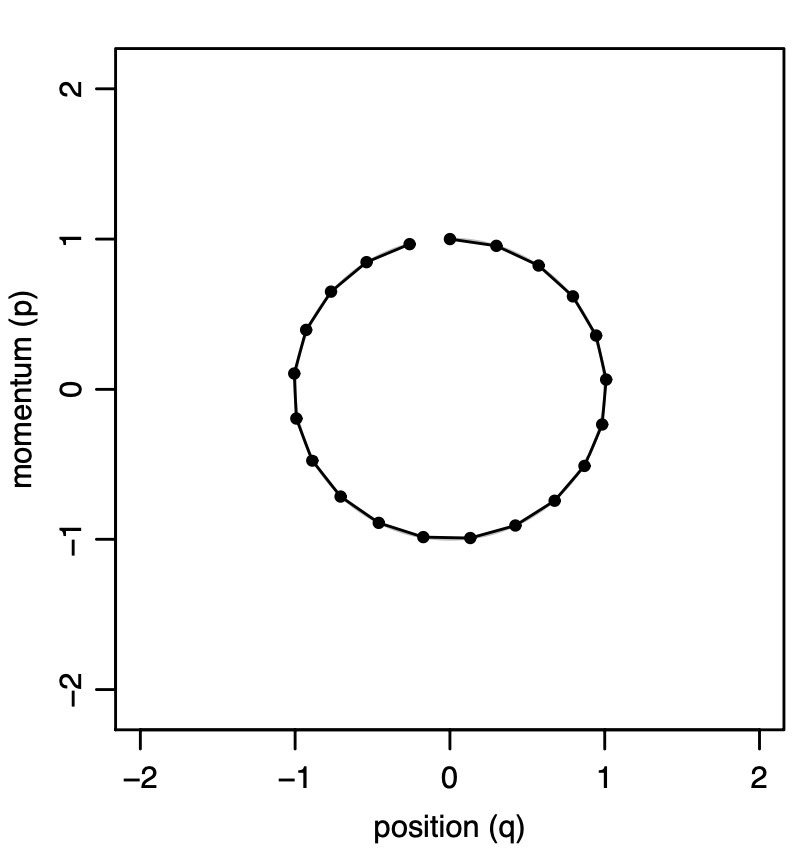
\includegraphics[width=0.8\columnwidth]{leapfrog_0_3.jpg}
				\caption{HMC numerically integrated using leapfrog with $\epsilon = 0.3$ and $L = 20$}
			\end{figure}
		\end{column}
	\end{columns}
\end{frame}

% \begin{frame}{An Interlude into Numerical Integration}
% 	In the field of ordinary differential equations (ODE),
% 	we have the idea of ``discretizing'' a system of ODEs by applying a
% 	small step-size $\epsilon$\footnote{sometimes also called $h$}.
% 	Such approaches are called \textbf{numerical integrators} and are composed by
% 	an ample class of tools.
% 	\vfill
% 	The most famous and simple of these numerical integrators is the Euler method,
% 	where we use a step-size $\epsilon$ to compute a numerical solution of system
% 	in a future time $t$ from specific initial conditions.
% \end{frame}

% \begin{frame}{An Interlude into Numerical Integration}
% 	\begin{columns}
% 		\begin{column}{0.6\textwidth}
% 			The problem is that Euler method, when applied to Hamiltonian dynamics,
% 			\textbf{does not preserve volume}.
% 			One of the fundamental properties of Hamiltonian dynamics if
% 			\textbf{volume preservation}\footnotemark.
% 			This makes the Euler method a bad choice as a HMC's numerical integrator.
% 		\end{column}
% 		\begin{column}{0.4\textwidth}
% 			\begin{figure}
% 				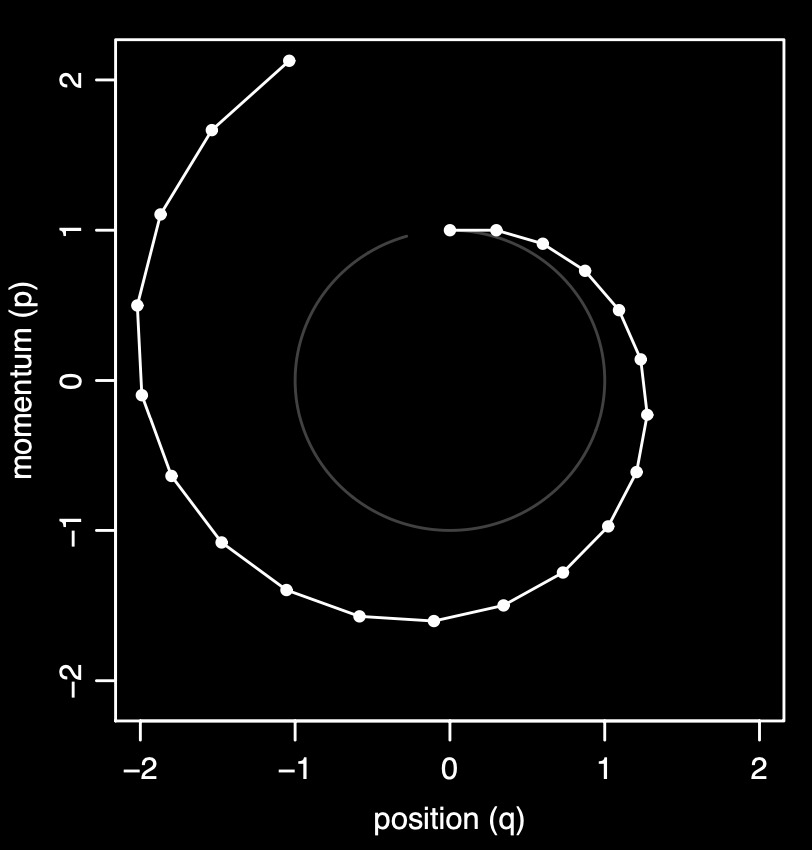
\includegraphics[width=0.8\columnwidth]{euler_0_3.jpg}
% 				\caption{HMC numerically integrated using Euler with $\epsilon = 0.3$ and $L = 20$}
% 			\end{figure}
% 		\end{column}
% 	\end{columns}
% 	\footnotetext{a result called Liouville theorem.}
% \end{frame}

% \begin{frame}{An Interlude into Numerical Integration\footnote{
% 			An excellent textbook for numerical and symplectic integrator is
% 			\textcite{irseles2008numericalanalysis}.}}
% 	\begin{columns}
% 		\begin{column}{0.6\textwidth}
% 			To preserve volume, we need a numerical \textbf{symplectic integrator}.
% 			Symplectic integrators are at most second-order
% 			and demands a constant step-size $\epsilon$.
% 			One of the main numerical symplectic integrator used
% 			in Hamiltonian dynamics is the \textbf{Störmer–Verlet integrator},
% 			also known as \textbf{leapfrog integrator}.
% 		\end{column}
% 		\begin{column}{0.4\textwidth}
% 			\begin{figure}
% 				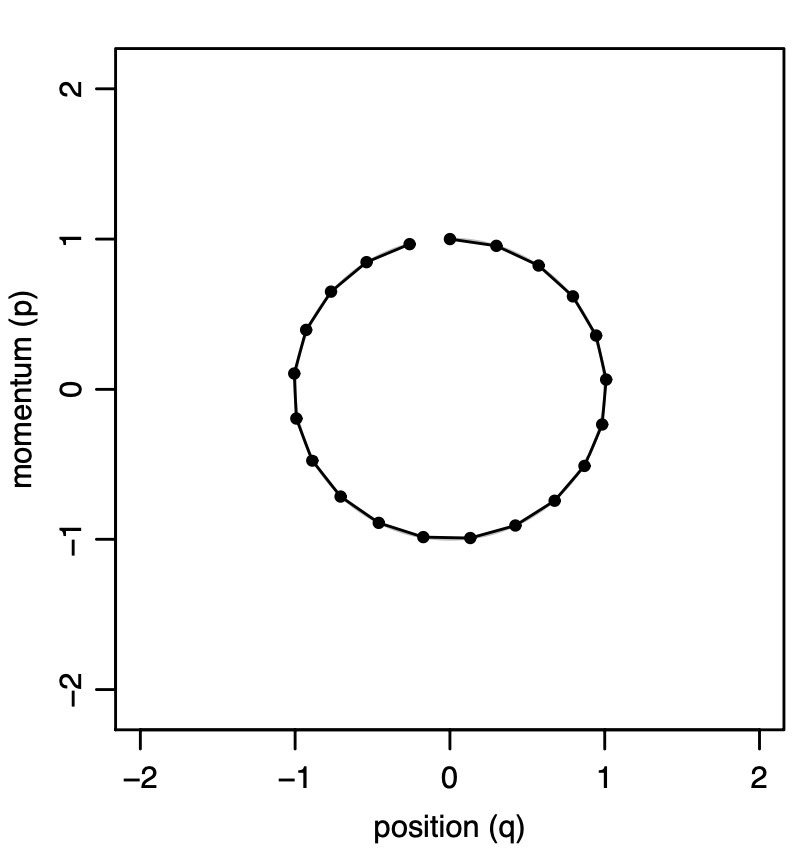
\includegraphics[width=0.8\columnwidth]{leapfrog_0_3.jpg}
% 				\caption{HMC numerically integrated using leapfrog with $\epsilon = 0.3$ and $L = 20$}
% 			\end{figure}
% 		\end{column}
% 	\end{columns}
% \end{frame}

\begin{frame}{Limitations of the HMC Algorithm}
	\begin{columns}
		\begin{column}{0.6\textwidth}
			As you can see, HMC algorithm is highly sensitive to the choice of
			leapfrog steps $L$ and step-size $\epsilon$,
			More specific, the leapfrog integrator allows only a constant $\epsilon$.
			There is a delicate balance between $L$ and $\epsilon$,
			that are hyperparameters and need to be carefully adjusted.
		\end{column}
		\begin{column}{0.4\textwidth}
			\begin{figure}
				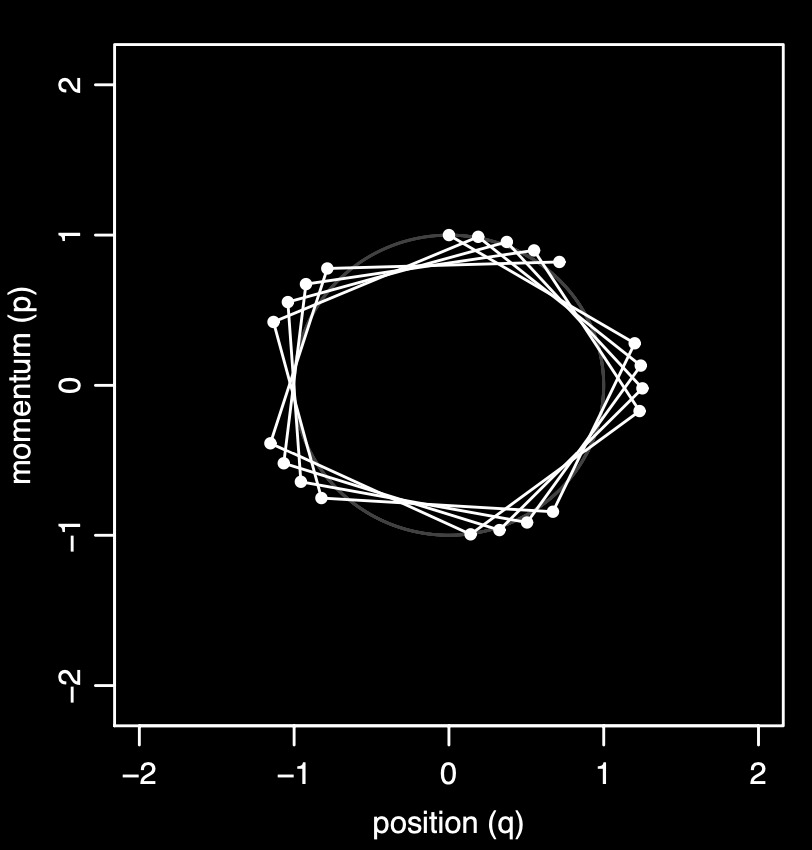
\includegraphics[width=0.8\columnwidth]{leapfrog_1_2.jpg}
				\caption{HMC numerically integrated using leapfrog with $\epsilon = 1.2$ and $L = 20$}
			\end{figure}
		\end{column}
	\end{columns}
\end{frame}

\subsubsection{No-U-Turn-Sampler (NUTS)}
\begin{frame}{\textbf{N}o-\textbf{U}-\textbf{T}urn-\textbf{S}ampler (NUTS)}
	In HMC, we can adjust $\epsilon$ during the algorithm runtime.
	But, for $L$, we need to to ``dry run'' the HMC sampler to find a good candidate value for $L$.
	\vfill
	Here is where the idea for \textbf{N}o-\textbf{U}-\textbf{T}urn-\textbf{S}ampler (NUTS)
	\parencite{hoffman2014no} enters:
	you don't need to \textbf{adjust anything},
	just ``press the button''.
	It will automatically find $\epsilon$ and $L$.
\end{frame}

\begin{frame}{\textbf{N}o-\textbf{U}-\textbf{T}urn-\textbf{S}ampler (NUTS)}
	More specifically, we need a criterion that informs that we performed
	enough Hamiltonian dynamics simulation.
	In other words, to simulate past beyond would not increase the distance
	between the proposal $\boldsymbol{\theta}^{(*)}$ and the current value $\boldsymbol{\theta}$.
	\vfill
	NUTS uses a criterion based on the dot product between the current momenta vector
	$\boldsymbol{\phi}$ and the difference between the proposal vector $\boldsymbol{\theta}^{(*)}$
	and the current vector $\boldsymbol{\theta}$,
	which turns into the derivative with respect to time $t$ of half of the distance squared between
	$\boldsymbol{\theta}$ e $\boldsymbol{\theta}^{(*)}$:
	$$
		(\boldsymbol{\theta}^{(*)} - \boldsymbol{\theta}) \cdot \boldsymbol{\phi}
		= (\boldsymbol{\theta}^{(*)} - \boldsymbol{\theta}) \cdot \frac{d}{dt} (\boldsymbol{\theta}^{(*)} - \boldsymbol{\theta})
		= \frac{d}{dt} \frac{(\boldsymbol{\theta}^{(*)} - \boldsymbol{\theta}) \cdot (\boldsymbol{\theta}^{(*)} - \boldsymbol{\theta})}{2}
	$$
\end{frame}

\begin{frame}{\textbf{N}o-\textbf{U}-\textbf{T}urn-\textbf{S}ampler (NUTS)}
	This suggests an algorithms that does not allow proposals be guided infinitely
	until the distance between the proposal $\boldsymbol{\theta}^{(*)}$ and the current
	$\boldsymbol{\theta}$ is less than zero.
	\vfill
	This means that such algorithm will \textbf{not allow u-turns}.
\end{frame}

\begin{frame}{\textbf{N}o-\textbf{U}-\textbf{T}urn-\textbf{S}ampler (NUTS)}
	NUTS uses the leapfrog integrator to create a binary tree where each leaf node
	is a proposal of the momenta vector $\boldsymbol{\phi}$ tracing both a forward
	($t+1$) as well as a backward ($t-1$) path in a determined fictitious time $t$.
	The growing of the leaf nodes are \textbf{interrupted} when an u-turn is detected,
	both forward or backward.
	% \begin{figure}
	% 	\centering
	% 	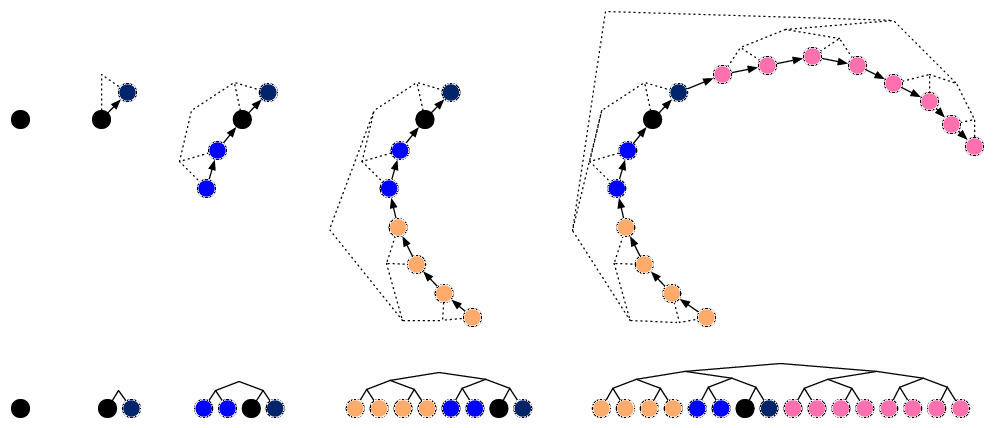
\includegraphics[width=0.6\textwidth]{nuts.jpg}
	% 	\caption{NUTS growing leaf nodes forward}
	% \end{figure}
\end{frame}

\begin{frame}{\textbf{N}o-\textbf{U}-\textbf{T}urn-\textbf{S}ampler (NUTS)}
	NUTS also uses a procedure called Dual Averaging
	\parencite{nesterov2009primal} to simultaneously adjust $\epsilon$ and $L$
	by considering the product $\epsilon \cdot L$.
	\vfill
	Such adjustment is done during the warmup phase and the defined values of
	$\epsilon$ and $L$ are kept fixed during the sampling phase.
\end{frame}

\begin{frame}{NUTS Algorithm}
	\SetAlCapFnt{\footnotesize}
	\SetAlCapNameFnt{\footnotesize}
	\begin{algorithm}[H]
		\DontPrintSemicolon
		\SetAlgoNoEnd
		\SetAlgoLined
		\fontsize{4.5pt}{6.5pt}\selectfont
		Define an initial set $\boldsymbol{\theta}^{(0)} \in \mathbb{R}^p$ that $P\left(\boldsymbol{\theta}^{(0)} \mid \mathbf{y} \right) > 0$\;
		\textcolor{blue}{Instantiate an empty binary tree with $2^L$ leaf nodes}\;
		Sample $\boldsymbol{\phi}$ from a $\text{Multivariate Normal}(\mathbf{0},\mathbf{M})$\;
		Simultaneously sample $\boldsymbol{\theta}$ and $\boldsymbol{\phi}$ with $L$ leapfrog steps and step-size $\epsilon$.\;
		Define the current value $\boldsymbol{\theta}$ as the proposed value $\boldsymbol{\theta}^{(*)}$:
		$\boldsymbol{\theta}^{(*)} \leftarrow \boldsymbol{\theta}$\;
		\For{$1, 2, \dots, 2L$}{
			\textcolor{blue}{Choose a direction $v \sim \text{Uniform}\left( \left\{-1, 1 \right\} \right)$}\;
			Use the gradient of the $\log$ posterior $\boldsymbol{\theta}^{(*)}$ for a half-step of $\boldsymbol{\phi}$ in the direction $v$:
			$\boldsymbol{\phi} \leftarrow \boldsymbol{\phi} + v \frac{1}{2} \epsilon \frac{d \log P(\boldsymbol{\theta}^{(*)} \mid \mathbf{y})}{d \theta}$\;
			Use $\boldsymbol{\phi}$ to update $\boldsymbol{\theta}^{(*)}$:
			$\boldsymbol{\theta}^{(*)} \leftarrow \boldsymbol{\theta}^{(*)} + \epsilon \mathbf{M}^{-1} \boldsymbol{\phi}$\;
			Again use the gradient of the $\log$ posterior $\boldsymbol{\theta}^{(*)}$ for a half-step of $\boldsymbol{\phi}$ in the direction $v$:
			$\boldsymbol{\phi} \leftarrow \boldsymbol{\phi} + v \frac{1}{2} \epsilon \frac{d \log P(\boldsymbol{\theta}^{(*)} \mid \mathbf{y})}{d \theta}$\;
			Define the node $L_t^v$ as the proposal $\boldsymbol{\theta}$\;
			\If{
				The difference between proposal vector $\boldsymbol{\theta}^{(*)}$
				and current vector $\boldsymbol{\theta}$ in the direction $v$ is lower than zero: $v \frac{d}{dt} \frac{(\boldsymbol{\theta}^{(*)} - \boldsymbol{\theta}^{(*)}) \cdot (\boldsymbol{\theta}^{(*)} - \boldsymbol{\theta}^{(*)})}{2} < 0$\;
			}{
				\textcolor{red}{Stop sampling $\boldsymbol{\theta}^{(*)}$ in the direction $v$ and continue sampling only in the direction $-v$}\;
			}{
				\If{
					The difference between proposal vector $\boldsymbol{\theta}^{(*)}$
					and current vector $\boldsymbol{\theta}$ in the direction $-v$ is lower than zero: $-v \frac{d}{dt} \frac{(\boldsymbol{\theta}^{(*)} - \boldsymbol{\theta}^{(*)}) \cdot (\boldsymbol{\theta}^{(*)} - \boldsymbol{\theta}^{(*)})}{2} < 0$\;
				}{
					\textcolor{red}{Stop sampling $\boldsymbol{\theta}^{(*)}$\;
					}
				}
			}
		}
		As an acceptance/rejection rule, compute:
		$r = \frac{P \left(\boldsymbol{\theta}^{(*)} \mid \mathbf{y} \right) P \left(\boldsymbol{\phi}^{(*)} \right)}{P \left(\boldsymbol{\theta}^{(t-1)} \mid \mathbf{y} \right) P \left(\boldsymbol{\phi}^{(t-1)} \right)}$\;
		Assign:
		$
			\boldsymbol{\theta}^{(t)} =
			\begin{cases}
				\boldsymbol{\theta}^{(*)}   & \text{with probability $\min(r,1)$} \\
				\boldsymbol{\theta}^{(t-1)} & \text{otherwise}
			\end{cases}
		$\;
		\caption{No-U-Turn-Sampler (NUTS)}
	\end{algorithm}
\end{frame}

% \begin{frame}{NUTS Animation\footnote{see NUTS in action at \href{https://chi-feng.github.io/mcmc-demo/app.html?algorithm=EfficientNUTS&target=banana}{\texttt{chi-feng/mcmc-demo}}.}}
% 	\centering
% 	\movie[loop, width=9cm, height=6cm]{NUTS Animation}{animations/nuts.m4v}
% \end{frame}

\begin{frame}{NUTS Animation}
	See NUTS in action at \href{https://chi-feng.github.io/mcmc-demo/app.html?algorithm=EfficientNUTS&target=banana}{\texttt{chi-feng/mcmc-demo}}.
\end{frame}

\subsubsection{Limitations of HMC and NUTS}
\begin{frame}{Limitations of HMC and NUTS Algorithms -- \textcite{nealSliceSampling2003}'s Funnel}
	The famous ``Devil's Funnel''\footnote{very common in hierarchical models.}.
	Here we see that HMC and NUTS, during the exploration of the posterior,
	have to change often $L$ and $\epsilon$ values\footnote{
		remember that $L$ and $\epsilon$ are defined in the warmup phase and kept fixed during sampling.}.
	% https://crackedbassoon.com/writing/funneling
	% import numpy as np
	% import matplotlib
	% import matplotlib.pyplot as plt
	% from matplotlib import rcParams
	% from scipy.stats import norm
	% fs = rcParams["figure.figsize"]
	% rcParams["figure.figsize"] = (fs[0], fs[0] / 2)
	% rcParams["lines.linewidth"] = 2
	% rcParams["font.size"] = 14
	% rcParams["axes.edgecolor"] = 'b'
	% rcParams["xtick.labelcolor"] = 'w'
	% rcParams["ytick.labelcolor"] = 'w'


	% # generate data
	% np.random.seed(0)
	% k = 9
	% n = 10000
	% v = norm.rvs(0, 3, n)
	% x = norm.rvs(0, np.exp(v / 2), (k, n))

	% # plot data and analytic log-likelihood
	% r = 500
	% x, v = np.meshgrid(np.linspace(-20, 20, r), np.linspace(-9, 9, r))
	% logp = norm.logpdf(v, 0, 3) + norm.logpdf(x, 0, np.exp(v / 2))
	% plt.imshow(logp, vmin=-7.5, vmax=-2.5, cmap="viridis", origin="lower")
	% plt.xticks(np.linspace(0, 499, 5), labels=np.linspace(-20, 20, 5).astype(int))
	% plt.yticks(np.linspace(0, 499, 5), labels=np.linspace(-9, 9, 5).astype(int))

	% # save figure
	% plt.savefig('slides/images/funnel.png', bbox_inches=0, transparent=True, dpi=300)
	\centering
	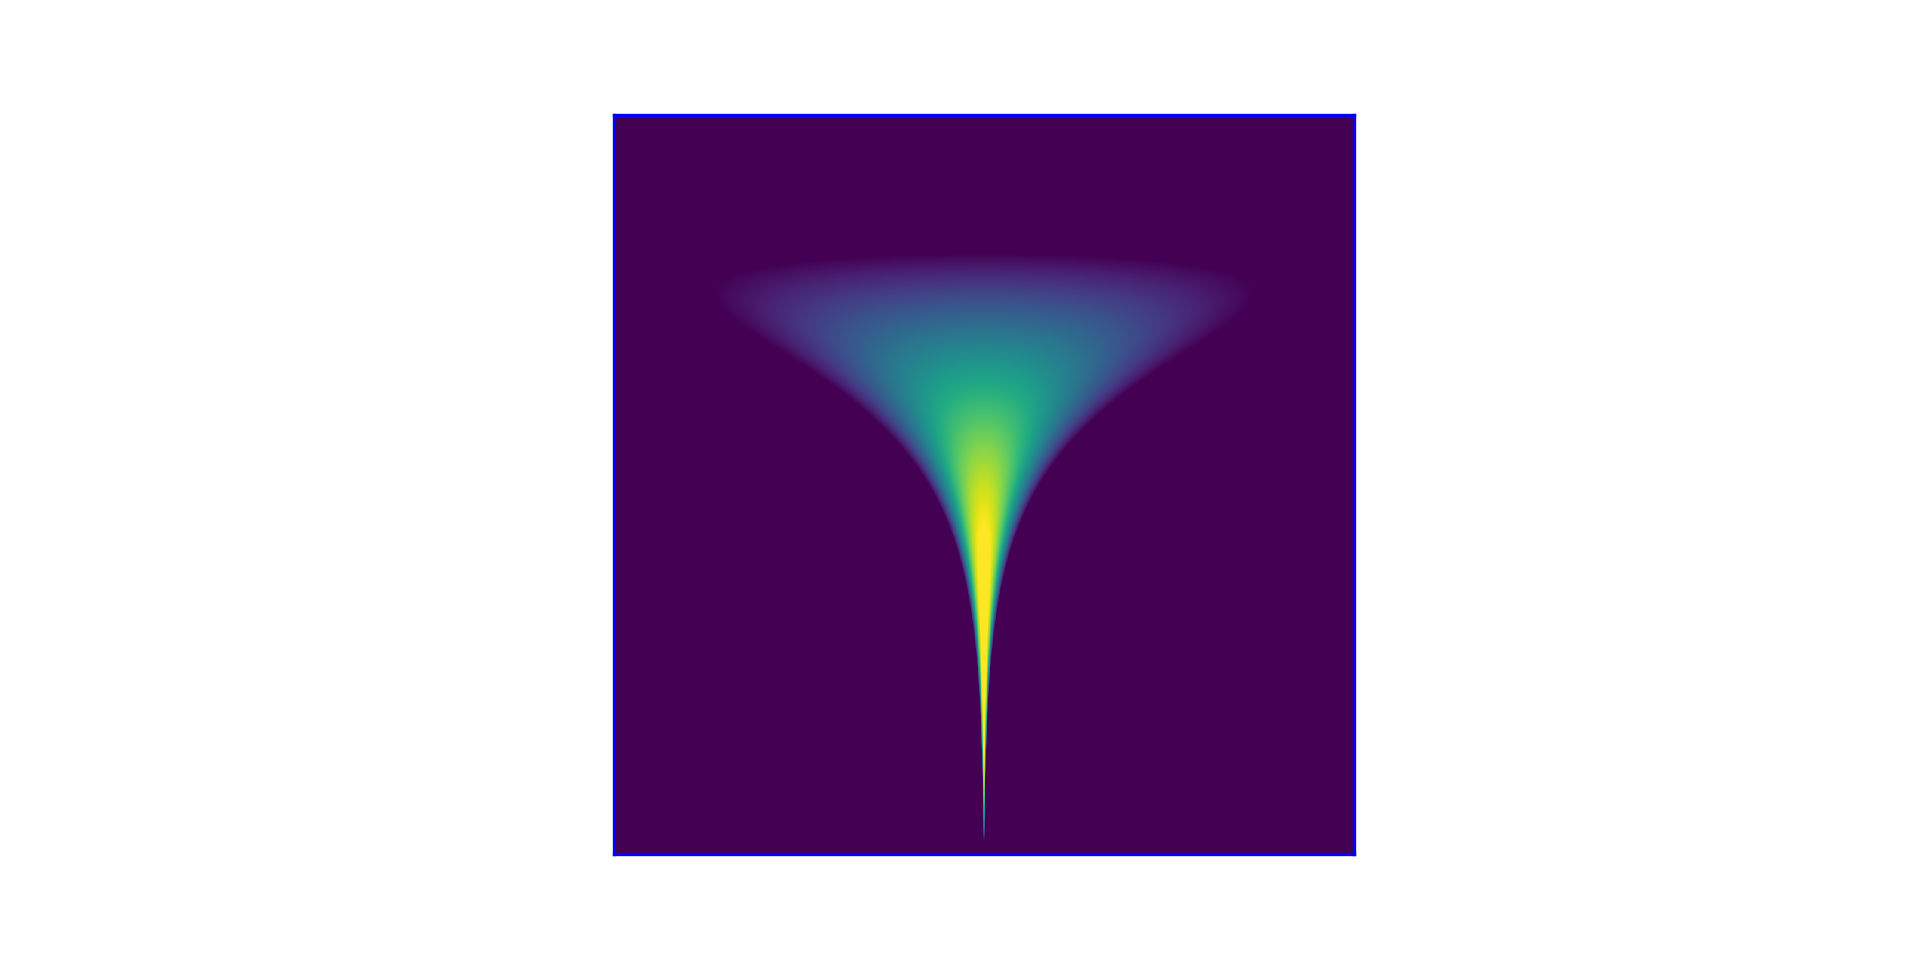
\includegraphics[width=0.65\textwidth]{funnel.png}
\end{frame}

\begin{frame}{\textcite{nealSliceSampling2003}'s Funnel and Non-Centered Parameterization (NCP)}
	Sometimes the group-level effects do not constrain the hierarchical distribution tightly.
	\vfill
	Examples arise when there are not many groups,
	or when the inter-group variation is high.
	\vfill
	In such cases, hierarchical models can be made much more efficient by shifting the
	data's correlation with the parameters to the hyperparameters.
\end{frame}

\begin{frame}{\textcite{nealSliceSampling2003}'s Funnel and Non-Centered Parameterization (NCP)}
	\small
	The funnel occurs when we have a variable that its variance depends on another variable variance
	in an exponential scale.
	A canonical example of a centered parameterization (CP) is:
	$$
		P(y,x) = \text{Normal}(y \mid 0 ,3) \cdot
		\text{Normal}\left(x \mid 0, e^{\left(\frac{y}{2}\right)}\right)
	$$
	This occurs often in hierarchical models,
	in the relationship between group-level priors and population-level hyperpriors.
	Hence, we reparameterize in a non-centered way,
	changing the posterior geometry to make life easier for our MCMC sampler:
	$$
		\begin{aligned}
			P(\tilde{y},\tilde{x}) & = \text{Normal}(\tilde{y} \mid 0, 1) \cdot
			\text{Normal}(\tilde{x} \mid 0, 1)                                           \\
			y                      & = \tilde{y} \cdot 3 + 0                             \\
			x                      & = \tilde{x} \cdot  e^{\left(\frac{y}{2}\right)} + 0
		\end{aligned}
	$$
\end{frame}

\subsection{More Intuition}
\begin{frame}{More Intuition - Step Size and Acceptance Ratio}
	\begin{vfilleditems}
		\item The NUTS algorithm adapts its stepping algorithm to encourage a certain fraction of the proposals to get accepted on average.
		\item A value of 0.99 means that we want to accept 99\% of the proposals the sampler makes.
		\item This will generally lead to small step sizes between the proposal and the current sample since this increases the chance of accepting such a proposal.
	\end{vfilleditems}
\end{frame}

\begin{frame}{More Intuition - Step Size and Acceptance Ratio}
	\begin{vfilleditems}
		\item On the other hand, a target acceptance fraction of 0.2 means that we want to only accept 20\% of the proposals made on average.
		\item The NUTS algorithm will therefore attempt larger step sizes to ensure it rejects 80\% of the proposals.
		\item In general, a target acceptance ratio value of 0.6-0.8 is recommended to use.
	\end{vfilleditems}
\end{frame}

\begin{frame}{More Intuition - Exploration vs Exploitation}
	\begin{vfilleditems}
		\item In sampling, there is usually a tradeoff between exploration and exploitation.
		\item If the sampler is too ``adventurous'', trying aggressive proposals that are far from the previous sample in each step, the sampler would be more likely to explore the full posterior and not get stuck sampling near a local mode of the posterior.
		\item However on the flip side, too much exploration will often lead to many sample rejections due to low joint probability of the data and the adventurous proposals. This can decrease the ratio of the effective sample size (ESS) to the total number of samples (aka relative ESS) since a number of samples will be mere copies of each other due to rejections.
	\end{vfilleditems}
\end{frame}

\begin{frame}{More Intuition - Exploration vs Exploitation}
	On the other hand if we do less exploration, there are 2 possible scenarios:
	\begin{vfilleditems}
		\item The first scenario is if we initialize the sampler from a mode of the posterior.
		\begin{vfilleditems}
			\item Making proposals only near the previous sample will ensure that we accept most of the samples.
			\item Proposals near a mode of the posterior are likely to be good parameter values.
			\item This local sampling behavior around known good parameter values is what we call exploitation.
			\item While the samples generated via high exploitation around a mode may not be representative of the whole posterior distribution, they might still give a satisfactory approximation of the posterior predictive distributions.
		\end{vfilleditems}
	\end{vfilleditems}
\end{frame}
\begin{frame}{More Intuition - Exploration vs Exploitation}
	\begin{vfilleditems}
		\item The second scenario is if we initialize the sampler from bad parameter values.
		\begin{vfilleditems}
			\item Bad parameter values and low exploration often lead to optimization-like behavior where the sampler spends a considerable number of iterations moving towards a mode in a noisy fashion.
			\item This optimization-like, mode-seeking behavior causes a high auto-correlation in the samples since the sampler is mostly moving in the same direction (towards the mode).
			\item A high auto-correlation means a low ESS because the samples would be less independent from each other.
			\item Also until the sampler reaches parameter values that actually fit the data well, it's unlikely these samples will lead to a good posterior predictive distribution.
		\end{vfilleditems}
	\end{vfilleditems}
\end{frame}
\begin{frame}{More Intuition - Exploration vs Exploitation}
	\begin{vfilleditems}
		\item The second scenario is if we initialize the sampler from bad parameter values.
		\begin{vfilleditems}
			\item This is a fairly common failure mode of MCMC algorithms when the adaptation algorithm fails to find a good stepping algorithm that properly explores the posterior distribution due to bad initial parameters and the model being too complicated and difficult to optimize, let alone sample from its posterior.
			\item In this case, all the samples may look auto-correlated and the step sizes between samples will likely be very small (low exploration).
			\item It's often helpful to detect such a failure mode early in the sampling and kill the sampling early.
		\end{vfilleditems}
	\end{vfilleditems}
\end{frame}
\begin{frame}{More Intuition - Mass Matrix, Adaptation and U-Turn}
	\begin{vfilleditems}
		\item The NUTS algorithm adapts the level of exploration in its proposal mechanism to achieve the target acceptance ratio.
		\item However, the definition of an ``exploratory'' proposal may be different depending on the parameter values of the current sample.
		\item For relatively flat regions of the posterior where a lot of parameter values are almost equally likely (i.e. they all the fit the data well and are almost equally probable according to the prior), proposals far away from the current sample may still be accepted most of the time.
		\item This is especially likely in the parts of the posterior where the model is non-identifiable or there are high parameter correlations, and the prior is indiscriminate (e.g. due to being a weak prior).
	\end{vfilleditems}
\end{frame}

\begin{frame}{More Intuition - Mass Matrix, Adaptation and U-Turn}
	\begin{vfilleditems}
		\item On the other hand, regions of the posterior that are heavily concentrated around a mode with a high curvature often require a smaller step size to achieve reasonable acceptance ratios.
		\item Proposals that are even slightly far from the current sample may be extremely improbable according to the prior or may lead to very bad predictions.
		\item This is especially likely in regions of the posterior where the model is highly sensitive to the parameter values or if the prior is too strongly concentrated around specific parameter values.
	\end{vfilleditems}
\end{frame}

\begin{frame}{More Intuition - Mass Matrix, Adaptation and U-Turn}
	\begin{vfilleditems}
		\item To account for such variation in curvature (wrt the same parameter in different regions), the NUTS algorithm uses a multi-step proposal mechanism with a fixed step size (determined during adaptation and then fixed) and a dynamic number of steps (dynamic in both adaptation and regular sampling).
		\item In other words, the sampler follows a trajectory of length $L \geq 1$ steps before proposing a new sample to move to, where $L$ is different in each proposal.
		\item This proposal then gets tested and is either accepted or rejected by comparing it to the previous sample.
	\end{vfilleditems}
\end{frame}

\begin{frame}{More Intuition - Mass Matrix, Adaptation and U-Turn}
	\begin{vfilleditems}
		\item The exact trajectory length taken by the NUTS sampler to propose a new sample is obtained by a binary tree search procedure with the maximum depth of the tree being a hyper-parameter of the algorithm.
		\item The goal of the tree search is to look for a point in the trajectory where a U-Turn happens, i.e. the sampler is beginning to trace back its steps.
		\item Once a U-turn is found, a point (randomly chosen) before the U-Turn becomes the next proposal and the search is terminated.
		\item This is typically considered a sign of successful exploration.
	\end{vfilleditems}
\end{frame}

\begin{frame}{More Intuition - Mass Matrix, Adaptation and U-Turn}
	\begin{vfilleditems}
		\item For some complicated models, the adaptation can often result in a step size that is too small.
		\item In such a case, no U-Turn may be found early and the tree search may have to run to completion before making a single proposal.
		\item If this happens in almost every iteration of the MCMC sampling, this will be bad for performance because the number of model evaluations required by a complete search tree of depth $d$ is $2^d - 1$.
	\end{vfilleditems}
\end{frame}

\begin{frame}{More Intuition - Mass Matrix, Adaptation and U-Turn}
	\begin{vfilleditems}
		\item The step size and trajectory length are not the only ways which the NUTS algorithm uses to adapt the level of exploration in the sampling.
		\item The so-called mass matrix (determined during adaptation and then fixed afterwards) allows the sampler to adapt the amount of exploration differently for different directions.
		\item This is especially important for models where parameters are on different scales so variables smaller in magnitude should generally be changing less between samples than variables larger in magnitude.
	\end{vfilleditems}
\end{frame}

\begin{frame}{More Intuition - Mass Matrix, Adaptation and U-Turn}
	\begin{vfilleditems}
		\item In Pumas, we use a diagonal mass matrix in \lstinline{BayesMCMC} (joint MCMC) where different exploration levels are used for different model parameters.
		\item If the mass matrix is dense (e.g. in \lstinline{MarginalMCMC}) (marginal MCMC), the exploration level can be different along arbitrary directions and not just along the parameters' axes.
		\item This tends to help when the parameters are heavily correlated in the posterior.
		\item The reason why it's called the mass matrix is an analogy to Hamiltonian dynamics that the HMC and NUTS algorithms were inspired from.
	\end{vfilleditems}
\end{frame}

\begin{frame}{\texttt{Stan} and NUTS}
	\texttt{Stan} was the first MCMC sampler to implement NUTS.
	Besides that, it has an automatic optimized adjustment routine for values of $L$ and $\epsilon$ during warmup.
	It has the following default NUTS hyperparameters' values\footnote{
		for more information about how to change those values, see \href{
			https://mc-stan.org/docs/reference-manual/hmc-algorithm-parameters.html}{
			Section 15.2 of the \texttt{Stan} Reference Manual}.}:
	\begin{vfilleditems}
		\item \textbf{target acceptance rate of Metropolis proposals}: 0.8
		\item \textbf{max tree depth}: 10
	\end{vfilleditems}
\end{frame}

\begin{frame}{\texttt{Pumas} and NUTS}
	\texttt{Pumas} also uses a NUTS implementation from the package \texttt{AdvancedHMC.jl}.
	It also has an automatic optimized adjustment routine for values of $L$ and $\epsilon$ during warmup that's identical to Stan's.
	It has the same default NUTS hyperparameters' values:
	\begin{vfilleditems}
		\item \textbf{target acceptance rate of Metropolis proposals}: 0.8
		\item \textbf{max tree depth}: 10
	\end{vfilleditems}
\end{frame}
